\chapter{Measurement of the realized circuit in the time domain}
\label{ch:measurement}
% The heart of the thesis, comprising a presentation of the functioning system and thus the culmination of the work. Important is an analysis of the results as well as a comparison with the state of the art. The reader should understand in this section why you should be awarded a MSc degree.

% to avoid unnecessary much heat and power losses. 

%The aim of the measurement was to show the feasibility to generate (different) signals, using the two bit resolution of the circuit.

The aim of the measurement was to show the generation of different signals.\\
With respect to produce a decent signal waveform at the output, the assembled hybrid test circuit was terminated with a \SI{50}{\ohm} termination and a \SI{3.3}{\nano\farad} capacitance, respectively.
In contrast to the calculated capacitance of \SI{20}{\pico \farad} in chapter \ref{ch:design}, an over dimensioned capacitor of \SI{3.3}{\nano\farad} terminated the output, to ensure that the signal would not be clipped.
%The assembled hybrid test circuit was measured with respect to produce a decent signal waveform at its output in the time domain.
%For the measurement (in the time domain) the output of the realized circuit was terminated with a \SI{50}{\ohm} termination and a \SI{3.3}{\nano\farad} capacitance, respectively.
%The output voltage waveform was measured with a \SI{50}{\ohm} termination and a \SI{3.3}{\nano\farad} capacitance, respectively.
%A discrete passive capacitor replaced the calculated impedance in chapter \ref{ch:design} used for the simulation.

After the calibration of the measurement instruments, a stability check was performed to ensure that the test circuit do not oscillate.
%Otherwise the circuit (would oscillate and) could damage the chips.
In a next step the output of the circuit was measured with a resistive load to show the function of the push-pull stage.
%For the input control voltage a \gls{ab:awg} from Keysight Technologies was used.
The correct functioning of the push-pull stage enabled the measurement with a capacitive load to synthesize a triangular waveform.
In order to avoid any kind of damage, the measurement was performed with low \gls{ab:dc} supply voltages.


\section{Measurement setup}
An overview of the measurement setup is given in Figure \ref{fig:SchematicMeasSetup}.\\
%To ensure the instruments to work properly without taking damage their specifications have to be complied.
%In order to get good measurement results some requirements have to be fulfilled.
%an overview of the measurement setup is given.
%In order to comply specification of the measurement instruments and avoid them to be damaged, it was necessary to fulfil some conditions.
A signal generator generated a square wave signal with an amplitude of \SI{0.7}{\volt} and \SI{0.45}{\volt}, respectively.
As a square wave signal consists of several harmonics, the pre amplifier had to support a wide bandwidth.\\
The square wave of $Ch1$ \& $\overline{Ch1}$ and $Ch2$ \& $\overline{Ch2}$ of the \gls{ab:awg} \cite{Keysight2015} is amplified by the broadband amplifier G1 and G2, respectively.\\
A \gls{ab:dc} bias voltage is applied to the inputs of the \gls{ab:dut} to generate a square wave signal from $V_{low}$ = \SI{-10}{\volt} to $V_{high}$ = \SI{-5}{\volt}.
The voltage swing of \SI{5}{\volt} as well as the \gls{ab:dc} bias voltage were needed, to ensure that the input transistors switch completely on and off.
%In order to ensure that the \gls{ab:hemt} base transistor at the input of the circuit is fully switched on and off a peak to peak value of \SI{5}{\volt} is needed.
%\SI{5}{\volt} peak to peak input signal is needed to ensure that the \gls{ab:hemt} is fully opened or fully closed.\\
Several power supplies provided the necessary \gls{ab:dc} supply voltages for the broadband amplifiers, bias tees and the \gls{ab:dut}.\\
For the measurement of the push-pull stage, an attenuator with \SI{20}{\decibel} attenuation was connected between the output of the \gls{ab:dut} and the input of the oscilloscope.
This attenuator ensured that the specifications of the oscilloscope (scope 1) were complied.\\
The measurement of the voltage across the load capacitance was done by another oscilloscope (scope 2) which provides a handy probe.
This probe allowed to measure the voltage directly on the output line of the hybrid test circuit.


\begin{figure}[htb!]
	\centering
  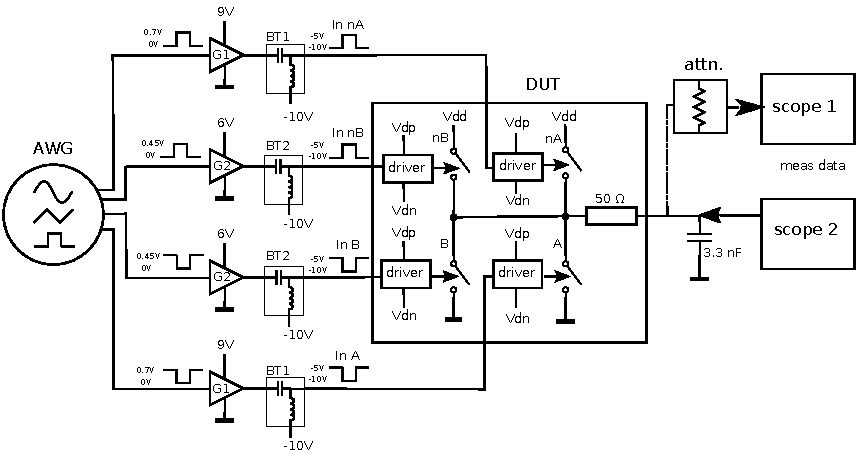
\includegraphics{meassetupschem.pdf}
	\caption{Schematic of time domain measurement setup}
	\label{fig:SchematicMeasSetup}
\end{figure}

%This signal is amplified by a pre power amplifier to get a decent voltage swing of \SI{5}{\volt}.
%This swing is needed to be sure to turn the \gls{ab:gan} \gls{ab:hemt} at the input of the circuit on and off.
%In addition to the swing another requirement is a \gls{ab:dc} offset of \SI{-10}{\volt}, because the transistor is a normally on device.
%The \gls{ab:dc} bias is fed through a bias tee to ensure that the output of the \gls{ab:awg} is not loaded.\\
%In fact that maximum input signal of the oscilloscope is at \SI{2}{\volt}, the signal provided by the circuit has to be attenuated.


The elements of the measurement setup were:
\begin{itemize}
	\item Signal generator: Keysight M8195A AWG
	\begin{itemize}
		\item $Ch1$ \& $\overline{Ch1}$: $V_{p-p}$ = \SI{0.7}{\volt} (square wave)
		\item $Ch2$ \& $\overline{Ch2}$: $V_{p-p}$ = \SI{0.45}{\volt} (square wave)
	\end{itemize}
	\item Broadband Amplifier
	\begin{itemize}
		\item G1: SHF803\\ gain = 17 dB (typ.), B = \SI{35}{\kilo \hertz} -  \SI{40}{\giga \hertz}
		\item G2: SHF804TL\\ gain = 21 dB (typ.), B = \SI{200}{\kilo \hertz} -  \SI{55}{\giga \hertz}
	\end{itemize}
	\item Bias Tee 
	\begin{itemize}
		\item BT1: SHF121A\\ B = \SI{50}{\kilo \hertz} -  \SI{65}{\giga \hertz}
		\item BT2: SHF121D\\ B = \SI{50}{\kilo \hertz} -  \SI{65}{\giga \hertz}
	\end{itemize}
	\item \gls{ab:dut}
	\item Power supplies
	\item Attenuator: 18B50W\\ B = \gls{ab:dc} -  \SI{18}{\giga \hertz}, Attenuation = 20 dB
	\item Capacitive load\\
	ceramic \gls{ab:smd} capacitor (\SI{3.3}{\nano \farad})
	\item Oscilloscope
	\begin{itemize}
		\item scope 1: DCA-X 86100D + 86118A (module)
		\item scope 2: DSO-X 3034A + HP 10432A (probe)
	\end{itemize}		
\end{itemize}

\begin{figure}[htb!]
	\centering
  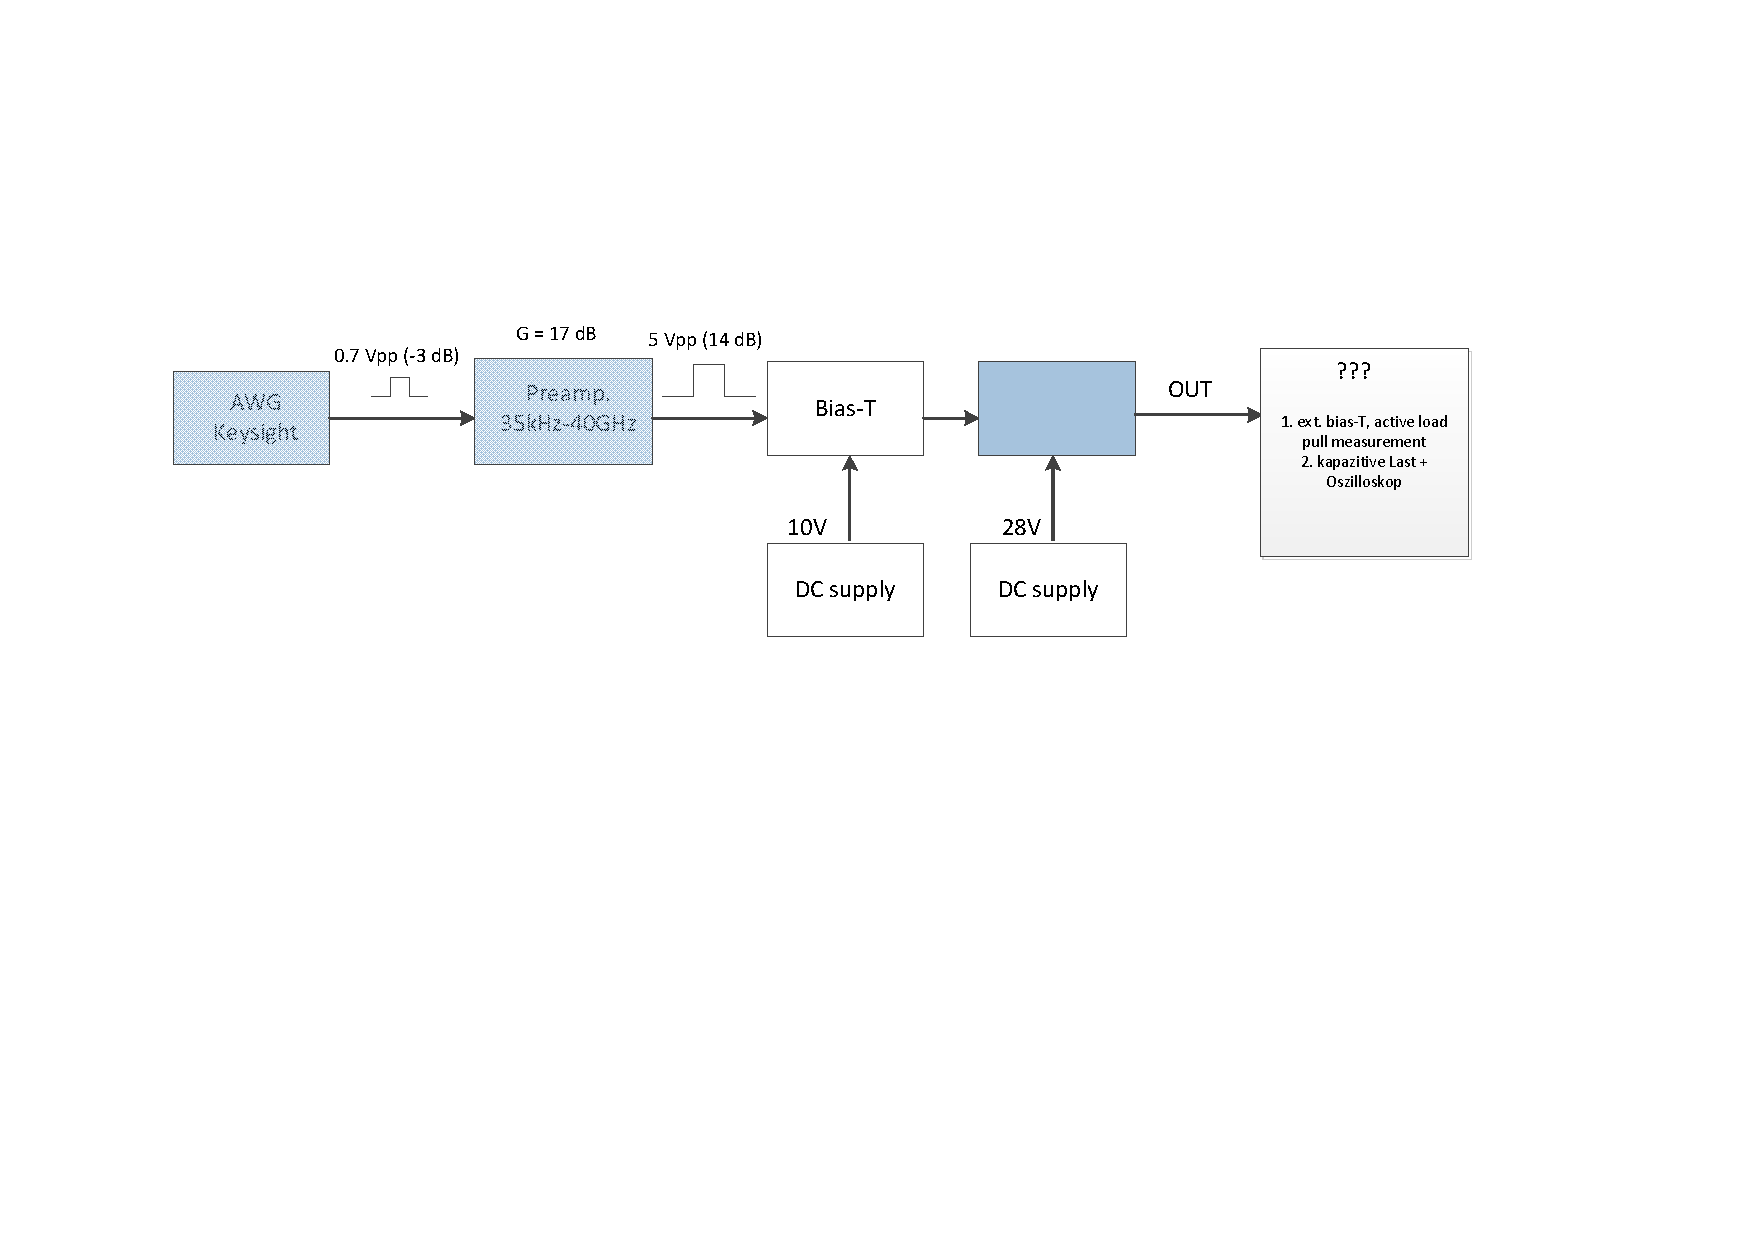
\includegraphics{MeasSetup.pdf}
	\caption{Photograph of measurement setup}
	\label{fig:PhotoMeasSetup}
\end{figure}

\section{Calibration and stability check}
Before performing the first measurement, the instruments and used devices had to be calibrated.
The \gls{ab:awg} output amplitude had to be adjusted to the proper value depending on which pre amplifier is used, as the broadband amplifiers differed in their gain.
The actual broadband amplifiers gain has to be checked as well as the proper configuration of the bias voltages.
These prerequisites are necessary to ensure a proper measurement.
After the calibration, the first measurement checked the stability of the circuit.
Therefore the \gls{ab:dut} was supplied with its bias voltages and the current was checked if it stays constant.
Due to the fact that the current was stabilized after the transient time, it showed that the circuit is stable.
For this measurement the in- and output connectors were terminated with \SI{50}{\ohm} terminations.\\
Simulation yielded a power consumption of \SI{1.29}{\watt} for the one-bit configuration using the smaller push pull stage.
This push pull stage is marked in the schematic in appendix \ref{app:schematicRealizedPump} with C and can be seen on the right side for landscape orientation of the schematic.
This smaller push pull stage refers to the stage B for the designed layout.
The built demonstrator yielded a power consumption of \SI{2.3}{\watt} for a switching frequency of \SI{200}{\mega \hertz} and $V_{dd} = 5V, V_{dn} = -5V, V_{dp} = 0V$.

\section{Time domain measurement of push-pull stage}
After checking the stability of the \gls{ab:dut}, the functionality was analysed.
A digital input signal was fed to the input of the device, to check the proper switching at the output.
Both inputs were controlled with a synchronous data signal so that both push pull stages switch synchronously either to \gls{sy:Vdd} or to \gls{ab:gnd}. % in phase signal
In between the commutation time, both power transistors, high and low side, were in the on state and thus the output is floating between \gls{sy:Vdd} and GND.
This led to distortions in the measured signal.
Figure \ref{fig:inputMeas} shows the square wave input control signal generated by an \gls{ab:awg} from Keysight Technologies \cite{Keysight2015}.

\begin{figure}[htb!]
	\centering
  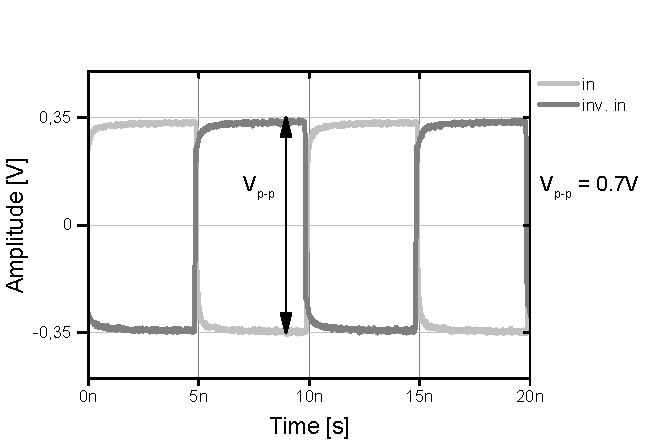
\includegraphics{inputVoltage.pdf}
	\caption{time domain measurement input control voltage}
	\label{fig:inputMeas}
\end{figure}

The square wave signal represents a digital data signal with a data rate of \SI{200}{Mbps} while the fundamental analog frequency is \SI{100}{\mega \hertz}.
In order to get a voltage swing of \SI{5}{\volt} at the input of the \gls{ab:dut} a peak to peak voltage of \SI{0.7}{\volt} was required.
This signal was pre amplified by the broadband amplifiers and an \gls{ab:dc} offset was added to ensure proper switching of the input control transistors.
The light grey signal represents one input stream while the darker grey signal represents the inverse one, respectively.
This signal represents the Riemann Code which was needed to control the circuit.
Using an alternating sequence of bits for both inputs, provides the output shown in figure \ref{fig:measRload100M}.

\begin{figure}[htb!]
	\centering
  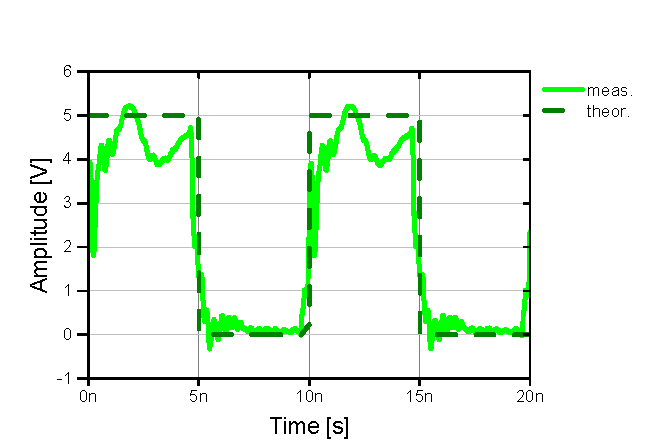
\includegraphics{100M_Rload_regression.pdf}
	\caption{Time domain measurement of output voltage with 50 Ohm termination}
	\label{fig:measRload100M}
\end{figure}

The circuit under test was terminated with an \SI{50}{\ohm} attenuator to avoid any damage to the oscilloscope (scope 1).
The light green signal presents the measured data while the dashed line describes the ideal behaviour.
In an ideal world there would be neither rising nor falling time and the signal would switch between logical one and zero.
As seen in Figure \ref{fig:measRload100M}, the output voltage switches between \gls{sy:Vdd} (here: \SI{5}{\volt}) and \gls{ab:gnd}. 
The measured signal shows fast rising and falling edges which demonstrates the abilitiy of fast switching. 
Due to measurement errors, process variations of the used components and parasitic effects the signal has some distortions.
Nevertheless the measured output signal proves the proper functioning of the realized test circuit.
The signal frequency matches with the digital input signal shown in figure \ref{fig:inputMeas}.

\section{Time domain measurement of synthesized signal}
\label{ch:timedomainmeas}
% to avoid any damage to the circuit, the power supply voltage was set to a very low value.
% in fact of the low value it was not ensurred that the transistors switch properly. this was a measurement erro....
% in adddition process variations come into play
% RC-element with 50 Ohm transmission line. Charge time reduce due to the occurence of the 50 Ohm environment. tau = R*C = 63% Vmax
%This differential input signal was needed to ensure proper switching of both bits.
Having demonstrated the proper functioning of the \gls{ab:dut} whereof both bits switched synchronous, it is shown that the circuit can synthesize signals with the resolution of two bits.
In fact of the two bit resolution the signals to generate were limited due to the restriction of four different slopes, as shown in Table \ref{tab:TwoBitRes}.

\begin{table}[]
\centering
\begin{tabular}{|l|l|l|}
\hline
\textbf{A} & \textbf{B} & \textbf{slope} \\ \hline
0          & 0          & $+3 i_0$          \\ \hline
0          & 1          & $+1 i_0$          \\ \hline
1          & 0          & $-1 i_0$          \\ \hline
1          & 1          & $-3 i_0$          \\ \hline
\end{tabular}
\caption{Encryption table for two bit resolution}
\label{tab:TwoBitRes}
\end{table}

In this measurement a capacitive load termination was needed which could demonstrate the different output currents $i_0$.
To avoid any damage to the measurement instruments and the \gls{ab:dut}, \gls{sy:Vdd} was set to \SI{5}{\volt} .
In order to avoid any signal clipping at the output, the capacitance was chosen to be \SI{3.3}{\nano \farad}.
Due to the fact that the output connector was terminated with a discrete \gls{ab:smd} capacitor a different measurement approach had to be considered.
For this measurement setup an oscilloscope with a probe head was chosen to analyse the signal at the capacitor.
The equivalent circuit for the measurement with the oscilloscope and a probe head is demonstrated in Figure \ref{fig:equivalentprobecircuit}.
\begin{figure}[htb!]
	\centering
  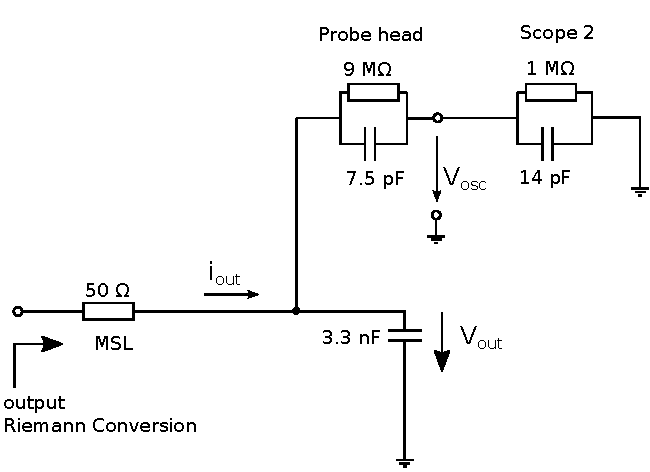
\includegraphics{ProbeMeasurementOsci2.pdf}
	\caption{equivalent circuit of the time domain measurement}
	\label{fig:equivalentprobecircuit}
\end{figure}

A drawback of this measurement process was that the probe head will load the output, which affects the measurement data.
Nevertheless this measurement was suitable to prove the concept of generating different signals.
The desired signals were two triangular waveforms generated with the slopes of $+3 i_0 / -3 i_0$ and $+1 i_0 / -1 i_0$.
This corresponds to an alternating input control sequence of 
\begin{equation}
 00\hspace{.3cm} 11\hspace{.3cm} 00\hspace{.3cm} 11\hspace{.3cm} [...],
\end{equation}
and
\begin{equation}
 01\hspace{.3cm} 10\hspace{.3cm} 01\hspace{.3cm} 10\hspace{.3cm} [...],
\end{equation}
respectively.
The data rate of the input signal was set to \SI{200}{Mbps} and \SI{300}{Mbps}, which yields a signal frequency of \SI{100}{\mega \hertz} and \SI{150}{\mega \hertz}.
The sequence representing the slope $3 i_0$ showed the expected behaviour from the push pull stage measurement.
Both inputs were controlled with a synchronous signal and hence both stages switched concurrently either to \gls{sy:Vdd} or to \gls{ab:gnd}.
In order to show that different signals could be synthesized a differential input signal was applied, which is demonstrated in Figure \ref{fig:inputMeas}.
This proof is shown in Figure \ref{fig:measCload100M}, as two triangular waveforms with different amplitudes could be synthesized.

\begin{figure}[htb!]
	\centering
  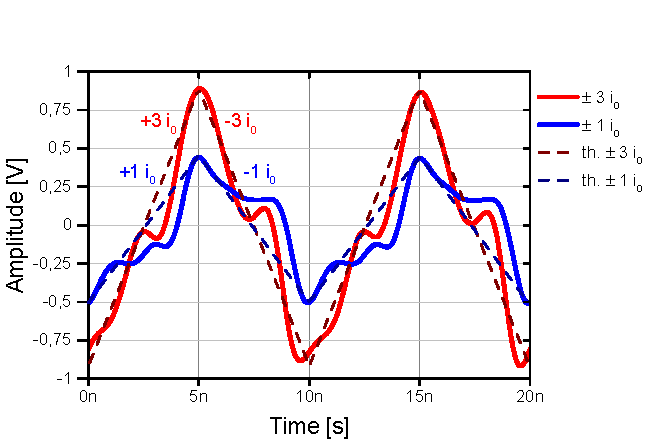
\includegraphics{100M_Cload_regression.pdf}
	\caption{time domain measurement with capacitive load at \gls{sy:fsignal} = 100MHz}
	\label{fig:measCload100M}
\end{figure}

The frequency of the synthesized signals is \SI{100}{\mega \hertz} while the voltage swing is \SI{1.8}{\volt} and \SI{0.8}{\volt} respectively.
The red signal represents a synthesized triangular waveform with a slope corresponding to $3 i_0$, while the brown dashed signal provides the ideal signal.
The signal corresponding to a slope of $1 i_0$ is marked blue, while the dashed dark blue signal provides the ideal signal waveform.
Further, signals were synthesized with an even higher frequency of \gls{sy:fsignal} = \SI{150}{\mega \hertz}.
For comparison purposes the notation was the same for the signals in figure \ref{fig:measCload150M}.

\begin{figure}[htb!]
	\centering
  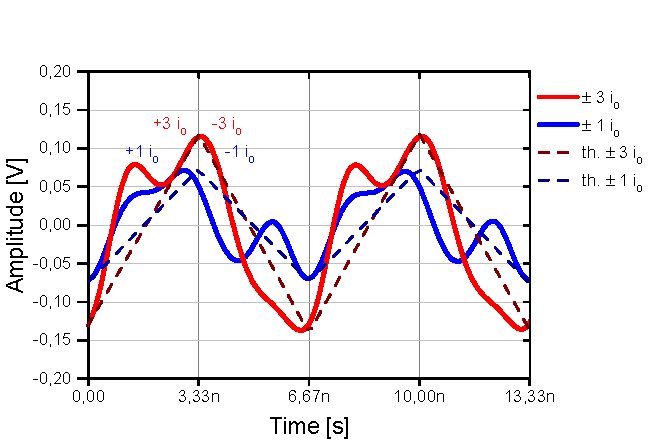
\includegraphics{150M_Cload_regression.pdf}
	\caption{time domain measurement with capacitive load at fs = 150MHz}
	\label{fig:measCload150M}
\end{figure}

In fact of the decreasing sampling interval for higher frequencies, the amplitudes of the signals are getting smaller, which is illustrated.
Also the difference between $3 i_0$ and $1 i_0$ is getting smaller and the same type of distortion become visible as for the former measurements.
Although the difference, between the amplitudes induced by $3 i_0$ and $1 i_0$, are getting smaller, the shape of a triangular signal can be interpreted.
Due to this effect and in addition to the visible distortions, an increase in frequency will lead to an unidentified signal.
Hence the \SI{150}{\mega \hertz} of \gls{sy:fsignal} was the upper bound on the frequency range in this measurement setup.
Because of the reduced supply voltage \gls{sy:Vdd} of \SI{5}{\volt}, the aspect of undefined current sources become visible, since the transistors do not operate in their saturation region.
Consequently the measured signals are distorted induced by undefined reference current source, commutation, leakage current and parasitic effects.
In fact of the limited scope of this thesis, a measurement was chosen to prove the concept, which was successful.
But this could have lead to measurement errors and deviations which should be reduced in future measurements.
The presented measurement results show the ability of generating different signals with the demonstrated concept.

\section{Discussion of measurement results}
In order to get meaningful measurement results a decent concept for the measurement set up had to be planned.
First of all, it was important to ensure the proper functioning of the inputs.
Therefore the right choice of broadband pre amplifier was indispensable.
A requirement for the pre amplifier was the broadband amplification, since square wave signals had to be amplified.
Secondly the right bias tees had to be chosen regarding the same broadband problematic.
After finding the right amplifiers and bias tees, the input control signal had to be calibrated to ensure the proper voltage swing to switch the \gls{ab:hemt} transistors on and off.
Depending on the desired measurement, the oscilloscope was chosen to get the time domain results.
In the first measurement an attenuator was needed to avoid any damage to the input of the oscilloscope.
Finding the right measurement instruments led to the expected results.
As presented, the switching of the push pull stage with both bits were successful.
After the verification that both power transistor were able to switch synchronous it was shown that both transistor could switch independently of each other and hence different output signals could be synthesized.
For the measurement for synthesizing a triangular waveform a different set up was needed.
Since the former measurement concept only showed the feasibility of switching the output either to \gls{sy:Vdd} or \gls{ab:gnd}, the second should demonstrate the ability to create different output signals.
In fact, it was shown that four different currents could be established, which corresponds to the theoretical achievable slopes.
This was shown by a capacitive load which was charged with these currents to obtain different output voltage waveforms.
It was possible to prove the demonstrated concept and show the feasibility of the designed demonstrator to synthesize signals with different amplitudes and frequencies.
The signal integrity suffered from measurement errors, non ideal switching and leakage currents.
Therefore the upper bound on the frequency range for the presented measurement setup with the realized circuit was at roughly \SI{150}{\mega \hertz}.
In addition to the undesired effects of the circuit topology, the problematic of the heat dissipation came into play.
Hence the signal integrity was reduced by the degradation induced by the heat.
Nevertheless, the results demonstrate for the first time the feasibility to convert digital signals into analog ones with the given concept and technology.
It was the first time ever, building a concrete test circuit in \gls{ab:gan} technology which provides decent measurement results.
Therefore it is to state, that the proof of concept was successfully demonstrated.